\documentclass{beamer}
\usepackage[utf8]{inputenc}
\usepackage[T1]{fontenc} 
\usepackage[slovene]{babel} 
\usepackage{lmodern}
\usepackage{amsfonts}  
\usepackage{mathtools}
\usepackage{amsmath}
\usepackage{amsthm} 

\newcommand{\R}{\mathbb R}
\newcommand{\N}{\mathbb N}
\newcommand{\Z}{\mathbb Z}
\newcommand{\C}{\mathbb C}
\newcommand{\Q}{\mathbb Q}
\newcommand{\overbar}[1]{\mkern 1.5mu\overline{\mkern-1.5mu#1\mkern-1.5mu}\mkern 1.5mu}


\usetheme{Warsaw}
\beamertemplatenavigationsymbolsempty
\setbeamertemplate{caption}[numbered]

\title{Schwarzov princip zrcaljenja za harmonične funkcije}
\author{Matej Novoselec}
\institute[UL FMF]{FMF Fakulteta za matematiko in fiziko}
\date{5. april 2023}


\theoremstyle{definition}
\newtheorem{defi}{Definicija}[section]
\theoremstyle{definition}
\newtheorem{op}[defi]{Opomba}
\newtheorem{trditev}{Trditev}
\newtheorem{lema}{Lema}
\newtheorem{izrek}{Izrek}

\begin{document}
%----------------------------------
\begin{frame}
   \titlepage
\end{frame}
%----------------------------------
\begin{frame}{Princip maksima}
   \begin{alertblock}{Princip maksima za holomorfne funkcije}
      Naj bo $D$ omejeno območje. Naj bo $h$ holomorfna na $D$ in zvezna na $\overline{D}$.
      Če velja $|h(z)| \leq M$ za vsak $z \in \partial D$, potem velja $|h(z)| \leq M$ za vsak $z \in \overline{D}$.
   \end{alertblock}  
\end{frame}
%----------------------------------
\begin{frame}{Dirichletov problem za enotski disk}
   \begin{alertblock}{Problem (Dirichletov problem za enotski disk)}
        Naj bo $\mathbb{D}$ enotski disk. Zvezno kompleksno funkcijo $h$, definirano na $\partial \mathbb{D}$, razširi do zvezne funkcije $\widetilde{h}$ tako, da bo $\widetilde{h}$ harmonična na $\mathbb{D}$ in zvezna na $\overline{\mathbb{D}}$, ter se bo zožitev $\widetilde{h}$ na $\partial \mathbb{D}$ ujemala s $h$.
   \end{alertblock}
   \pause
   \begin{exampleblock}{Spomnimo se...}
    Če razširitev obstaja je enolično določena.
    \pause
    \newline
    Oglejmo si enostavne zvezne funkcije.
   \end{exampleblock}
\end{frame}

\begin{frame}{Poissonovo jedro}
   \begin{block}{Definicija}
      \textbf{Poissonovo jedro} je funkcija definirana s predpisom
      $$
         P_r(\theta) = \sum_{k = -\infty}^{\infty}{r^{|k|} e^{i k \theta}}\text{, kjer je}~\theta \in [-\pi, \pi]~\text{in}~ r < 1.
      $$
   \end{block}
   \pause
   \begin{figure}
      \begin{center}
         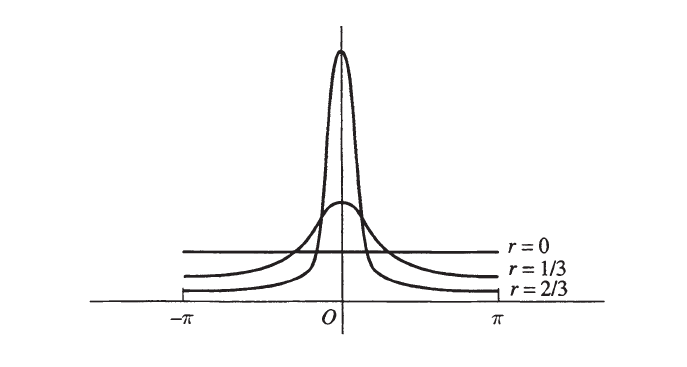
\includegraphics[width=0.70\textwidth]{poissonkernel.png}
      \end{center}
   \end{figure}
\end{frame}

\begin{frame}{Poissonov integral}
   \begin{block}{Definicija}
      \textbf{Poissonov integral}, ki ga označimo z~$\widetilde{h}(z)$, zvezne funkcije $h(e^{i\theta})$, je funkcija, definirana na enotskem disku s predpisom
      $$
      \widetilde{h}(z) = \int_{-\pi}^{\pi}{h(e^{i\varphi}) P_r(\theta - \varphi)~\frac{d\varphi}{2 \pi}}~\text{, kjer je}~~z = r e^{i\theta} \in \mathbb{D}.
      $$
   \end{block}
   \pause
   \begin{exampleblock}{Izrek (Poissonov integral)}
      Naj bo $h(e^{i \theta})$ zvezna funkcija na enotski krožnici. 
      Potem nam zgoraj definiran Poissonov integral $\widetilde{h}(z)$ ponuja razširitev funkcije $h$ do zvezne funkcije na $\overline{\mathbb{D}}$, harmonične v $\mathbb{D}$ in velja, da
      se njena zožitev na $\partial \mathbb{D}$ ujema s $h$.
   \end{exampleblock}
\end{frame}

\begin{frame}{Lastnost povprečne vrednosti}
   \begin{block}{Definicija} 
      Zvezna funkcija $h$, definirana na območju $D \subseteq \C$, ima \textbf{lastnost povprečne vrednosti}, če za vsak $z_0 \in D$ obstaja $\epsilon_0 > 0$, da je $\overline{\mathbb{D}}(z_0, \epsilon_0) \subseteq D$ in za vsak $0 < \epsilon \leq \epsilon_0 $ velja:
      $$
          h(z_0) = \frac{1}{2 \pi} \int_{0}^{2 \pi}{h(z_0 + \epsilon e^{i \theta}) d\theta}.
      $$
   \end{block}
   \pause
   \begin{exampleblock}{Izrek (Karakterizacija harmoničnih funkcij)}
      Naj bo $h(z)$ zvezna funkcija na območju $D$. 
      Potem je $h(z)$ harmonična na D natanko tedaj, ko ima $h(z)$ lastnost povprečne vrednosti na $D$.
   \end{exampleblock}
\end{frame}

\begin{frame}{Schwarzov princip zrcaljanja za harmonične funkcije}
   \begin{exampleblock}{Izrek (Schwarzov princip zrcaljenja za harmonične funckije)}
      Naj bo $D \subseteq \C$ območje, simetrično glede na realno os. 
      Označimo $D^{+} = D \cap \{\text{Im} > 0\}$ in $D^{-} = D \cap \{\text{Im} < 0\}$.
      \newline
      Naj bo $u(z): D^{+} \to \mathbb{R}$ harmonična funkcija, za katero velja, da gre $u(z) \to 0$, ko gre $z \in D^{+}$ proti poljubni točki $D \cap \mathbb{R}$ t.j.: $$\lim_{\text{Im}(z) \to 0^+} u(z) = 0.$$
      Potem obstaja harmonična razširitev $u(z)$ na $D$, ki jo podaja predpis $u(\bar{z}) = - u(z)$ za $z \in D$:
      $$
          u^e(z) = 
          \begin{cases}
              u(z)~~&z \in D^{+}\\
              -u(\overline{z})~~&z \in D^{-}\\
              0~~ &z \in \mathbb{R}
          \end{cases}
          .
      $$
   \end{exampleblock}
\end{frame}
\begin{frame}
   \begin{figure}
   \begin{center}
      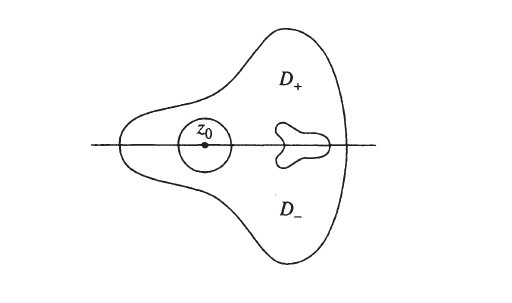
\includegraphics[width=0.90\textwidth]{schwarzov_princip_zrcaljenja.png}
   \end{center}
\end{figure}
\end{frame}

% -------------------------------------------------------------------
%---------------------------------------------------------
\end{document}
